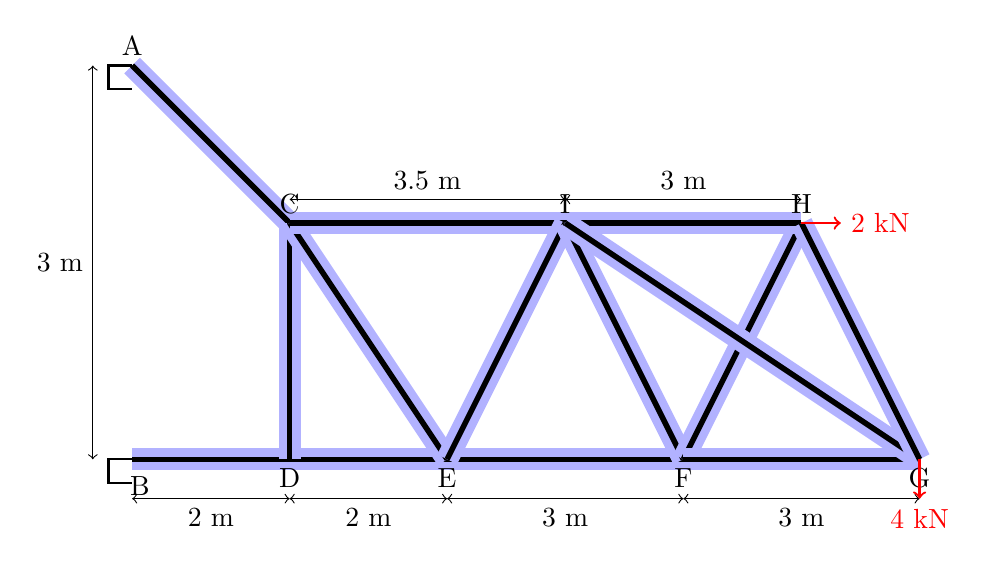
\begin{tikzpicture}
    \coordinate (A) at (0,5);
    \coordinate (B) at (0,0);
    \coordinate (C) at (2,3);
    \coordinate (D) at (2,0);
    \coordinate (E) at (4,0);
    \coordinate (I) at (5.5,3);
    \coordinate (F) at (7,0);
    \coordinate (H) at (8.5,3);
    \coordinate (G) at (10,0);
    \draw[line width=8pt, blue!30] (B) -- (D);
    \draw[line width=2pt, black] (B) -- (D);
    \draw[line width=8pt, blue!30] (D) -- (E);
    \draw[line width=2pt, black] (D) -- (E);
    \draw[line width=8pt, blue!30] (E) -- (F);
    \draw[line width=2pt, black] (E) -- (F);
    \draw[line width=8pt, blue!30] (F) -- (G);
    \draw[line width=2pt, black] (F) -- (G);
    \draw[line width=8pt, blue!30] (A) -- (C);
    \draw[line width=2pt, black] (A) -- (C);
    \draw[line width=8pt, blue!30] (C) -- (D);
    \draw[line width=2pt, black] (C) -- (D);
    \draw[line width=8pt, blue!30] (C) -- (E);
    \draw[line width=2pt, black] (C) -- (E);
    \draw[line width=8pt, blue!30] (C) -- (I);
    \draw[line width=2pt, black] (C) -- (I);
    \draw[line width=8pt, blue!30] (E) -- (I);
    \draw[line width=2pt, black] (E) -- (I);
    \draw[line width=8pt, blue!30] (I) -- (F);
    \draw[line width=2pt, black] (I) -- (F);
    \draw[line width=8pt, blue!30] (F) -- (H);
    \draw[line width=2pt, black] (F) -- (H);
    \draw[line width=8pt, blue!30] (G) -- (F);
    \draw[line width=2pt, black] (G) -- (F);
    \draw[line width=8pt, blue!30] (H) -- (I);
    \draw[line width=2pt, black] (H) -- (I);
    \draw[line width=8pt, blue!30] (I) -- (G);
    \draw[line width=2pt, black] (I) -- (G);
    \draw[line width=8pt, blue!30] (H) -- (G);
    \draw[line width=2pt, black] (H) -- (G);
    \draw[thick] (A) -- ++(-0.3,0) -- ++(0,-0.3) -- ++(0.3,0);
    \draw[thick] (B) -- ++(-0.3,0) -- ++(0,-0.3) -- ++(0.3,0);
    \node[above] at (A) {A};
    \node[below] at (0.1,-0.1) {B};
    \node[above] at (C) {C};
    \node[below] at (D) {D};
    \node[below] at (E) {E};
    \node[above] at (I) {I};
    \node[below] at (F) {F};
    \node[above] at (H) {H};
    \node[below] at (G) {G};
    \draw[<->, thin] (B)++(0,-0.5) -- node[below] {2 m} ++(2,0);
    \draw[<->, thin] (D)++(0,-0.5) -- node[below] {2 m} ++(2,0);
    \draw[<->, thin] (E)++(0,-0.5) -- node[below] {3 m} ++(3,0);
    \draw[<->, thin] (F)++(0,-0.5) -- node[below] {3 m} ++(3,0);
    \draw[<->, thin] (A)++(-0.5,0) -- node[left] {3 m} ++(0,-5);
    \draw[<->, thin] (C)++(0,0.3) -- node[above] {3.5 m} ++(3.5,0);
    \draw[<->, thin] (I)++(0,0.3) -- node[above] {3 m} ++(3,0);
    \draw[red, thick, ->] (H) -- ++(0.5,0) node[right] {2 kN};
    \draw[red, thick, ->] (G) -- ++(0,-0.5) node[below] {4 kN};
\end{tikzpicture}

